\chapter{Background}
  \section{Previous Work}
    \subsection{Defining the Internet of Things}
      The Internet of Things is a high-level concept which encompasses many ideas and technologies, and this makes it difficult to define absolutely. In this respect it is similar to Cloud Computing. Cloud Computing has come to represent different forms to different stakeholders, whether they are application developers, infrastructure engineers or end users. As the concept matured through research, conferences and industrial uptake, Cloud Computing has become identified by its use-cases and marketing jargon. For instance the industry has come to recognise Infrastructure-as-a-Service (IaaS), Platform-as-a-Service (PaaS) or Software-as-a-Service (Saas) as characteristics of the Cloud Computing concept \citep{viewOfCloud}. History may repeat itself with the Internet of Things where the definition will be refined as uptake and research improves.

      In the mean time we can begin plotting the footprint of IoT. The term `Internet of Things' captures the essence of the vision well; the vision of a world where everyday, physical objects are gateways to web-based services. These so-called `smart objects' comprise of sensors to perceive their environment or context, as well as a notion of inter-connectivity with other objects or services. Connected objects or services may react to collected data to trigger actions, and these actions may be digital or physical. The Internet of Things could be summarised as data collection, aggregation and reaction in the physical domain.

      The boundaries between IoT and other trends help to define its place in computing. For instance the research area of Wireless Sensor Networks (WSN) carries similarities in hardware requirements and challenges. In particular, WSN comprise of connected sensors and actuators \citep{Mottola:2011}. This differs from IoT because of the scope of connectivity; the closed-loop fashion of WSNs limit their potential to specific use-cases whereas the global context of IoT allows for a wider range of applications. Wireless Sensor Networks can form one layer of an Internet of Things application.

      The research area of `Wearables' also overlaps with the Internet of Things. Wearables are `smart' devices designed to be worn or embedded within the body and combine sensors and some form of connectivity, typically integrating with a smartphone \citep{6844949, evrything}. Consumer Wearables products are already on the shelves, such as Fitbit---a wrist-worn personal health tracker. The Fitbit wristband connects to a smartphone with Bluetooth Low Energy (BLE) and this smartphone then provides global connectivity through its wireless connection. Users can sign-in to a web-based dashboard which will collate and organise personal data. In this scenario, Wearables are collecting, aggregating and reacting to data in the physical domain. Wearables could therefore be decribed as a subset of the Internet of Things---they are an application in a specific domain.

      Two trends which acknowledge the vastness of information technology are `Ubiquitous Computing' and `Big Data'. The Ubiquitous Computing concept describes an environment where users are surrounded by connected technology---technology in our homes, workplaces and recreational activities. \cite{Weiser:1999} notes that ``specialized elements of hardware and software, connected by wires, radio waves and infrared, will be so ubiquitous that no one will notice their presence'' and this is reflective of the vision for Internet of Things. If Ubiquitous Computing describes a physical world saturated with sensors and devices then Big Data describes a \emph{digital} world saturated with huge datasets. These datasets will have different origins and so their structures may differ too; it is the purpose of Big Data to normalise and analyse these on a massive scale. The Internet of Things could be seen as a specific use case for both Ubiquitous Computing and Big Data.

      As we have seen, the boundary of the Internet of Things overlaps with other trends in computing. Figure \ref{iotRelationship} exemplifies the extent of which the definition of IoT relies on these related fields. What can be taken away about the definition of the Internet of Things is that it focuses on not just one idea or technology but rather a collection of them.

      \begin{figure}
        \centering
          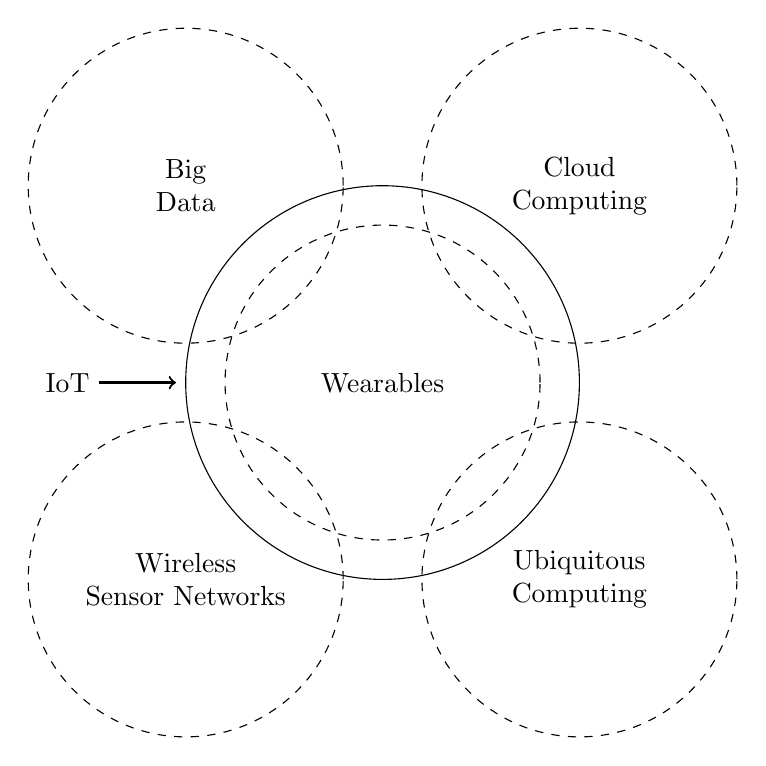
\begin{tikzpicture}
            \node (IoT) at (-2.5,0) {};
            \node at (-4,0) {IoT} edge[->,thick,out=0,in=180] (IoT);
            \draw (0,0) circle [radius=2.5];

            \node[align=center] at (0,0) {Wearables};
            \draw [dashed] (0,0) circle [radius=2];

            \node[align=center] at (-2.5,2.5) {Big\\Data};
            \draw [dashed] (-2.5,2.5) circle [radius=2];

            \node[align=center] at (2.5,2.5) {Cloud\\Computing};
            \draw [dashed] (2.5,2.5) circle [radius=2];

            \node[align=center] at (-2.5,-2.5) {Wireless\\Sensor Networks};
            \draw [dashed] (-2.5,-2.5) circle [radius=2];

            \node[align=center] at (2.5,-2.5) {Ubiquitous\\Computing};
            \draw [dashed] (2.5,-2.5) circle [radius=2];
          \end{tikzpicture}
        \caption{Describing the Internet of Things with other trends in computing}\label{iotRelationship}
      \end{figure}

    \subsection{Opportunities}
    \subsection{Challenges}
    \subsection{Use Cases}
  \section{Existing Platforms}
  \section{Sensor Hardware}
  \section{Platform Functions}
  \section{Case Studies}